\documentclass[aps,prl,amsmath,superscriptaddress]{revtex4}
\usepackage{graphicx}
\usepackage{color}
\usepackage{epstopdf}
\usepackage{xcolor}
\usepackage{sidecap}

\begin{document}

\title{Supplemental Material to "An individual Cr atom in a semiconductor quantum dot: optical addressability and spin-strain coupling"}

\author{A. Lafuente-Sampietro}
\affiliation{Universit\'{e} Grenoble Alpes, Institut N\'{e}el, F-38000 Grenoble, France}
\affiliation{CNRS, Institut N\'{e}el, F-38000 Grenoble, France}
\affiliation{Institute of Material Science, University of Tsukuba, Japan}

\author{H. Utsumi}
\affiliation{Institute of Material Science, University of Tsukuba, Japan}

\author{H. Boukari}
\affiliation{Universit\'{e} Grenoble Alpes, Institut N\'{e}el, F-38000 Grenoble, France}
\affiliation{CNRS, Institut N\'{e}el, F-38000 Grenoble, France}

\author{S. Kuroda}
\affiliation{Institute of Material Science, University of Tsukuba, Japan}

\author{L. Besombes}
\affiliation{Universit\'{e} Grenoble Alpes, Institut N\'{e}el, F-38000 Grenoble, France}
\affiliation{CNRS, Institut N\'{e}el, F-38000 Grenoble, France}


\begin{abstract}

In this supplemental material, we first describe the influence of strain on the fine structure of a Cr atom embedded in a II-VI zinc-blende semiconductor. We then present the complete electron-hole-Cr spin effective Hamiltonian used to model a low symmetry singly Cr-doped II-VI quantum dot. We finally present additional data on Cr-doped quantum dots: the temperature dependence of the PL of X-Cr and some statistics on the energy splitting of X-Cr and X$^2$-Cr.

\end{abstract}

\maketitle


\section{Cr energy levels in a II-VI semiconductor}

Cr atoms are incorporated into II-VI semiconductors as Cr$^{2+}$ ions on cation sites forming a deep impurity level. The ground state of a free Cr$^{2+}$ is $^{5}$D with the orbital quantum number L=2 and a spin S=2 yielding a 25-fold degeneracy. In the crystal field of T$_{d}$ symmetry of the tetrahedral cation site in zinc-blende crystal, the degeneracy is partially lifted (see Fig.~\ref{FigS1}): the $^{5}$D term splits into 15-fold degenerate orbital triplet $^{5}$T$_{2}$ and 10-fold degenerate orbital doublet $^{5}$E. The Jahn-Teller distortion reduces the symmetry to D$_{2d}$ and leads to a splitting of the $^{5}$T$_{2}$ ground state into a 5-fold degenerate $^{5}$B$_{2}$ orbital singlet and a $^{5}$E orbital doublet .

The ground state orbital singlet $^{5}$B$_{2}$ is further split by the spin-orbit interaction. In a strain free crystal, it was found that the ground state splitting can be described by the spin effective Hamiltonian \cite{Vallin1974}:

\begin{eqnarray}
\label{exchange} {\cal H}_{Cr,CF}=D_0S_z^2+\frac{1}{180}F[35S_z^2-30S(S+1)S_z^2+25S_z^2]+\frac{1}{6}a[S_1^4+S_2^4+S_3^4]
\end{eqnarray}

\noindent with the Cr spin S=2 and $|D_0|\gg|a|$, $|F|$. In the model presented here, we use $a=0$ and $F=0$. The x, y, z principal axes were found to coincide with the cubic axes (1,2,3) giving rise to three identical sites, each given by (\ref{exchange}) but with the z axis of each along a different cubic axis (1,2,3). A value of D$_0\approx+30 \mu eV$ was estimated from Electron Paramagnetic Resonance (EPR) measurements in highly diluted bulk (Cd,Cr)Te \cite{Vallin1974}.

\begin{figure}[hbt]
\includegraphics[width=3.0in]{FigS1.eps}
\caption{Scheme of the energy level splitting of Cr$^{2+}$ at a cation site in II-VI compounds having zinc blende structure (T$_d$) with a crystal field parameter $\Delta$, a Jahn-Teller energy E$_{J-T}$ and a spin-orbit level spacing D$_0$.}
\label{FigS1}
\end{figure}

Static biaxial compressive strain in the (001) plane, as observed in self-assembled quantum dots, reduces the symmetry to D$_{2d}$ and destabilize the Cr $3d$ orbitals $d_{xz}$ and $d_{yz}$ having an electron density pointing along the $[$001$]$ axis ($z$ axis). The Cr ground state is then a 5-fold degenerated orbital singlet formed from the $d_{xy}$ orbital. It corresponds to the Jahn-Teller ground state with a tetragonal distortion along the $[$001$]$ axis \cite{Brousseau1988}.

An applied stress will also  influence the Cr spin fine structure splitting through the modification of the crystal field and the spin-orbit interaction \cite{Vallin1974}. For an arbitrary strain tensor, the general form of the Cr ground state spin effective Hamiltonian is

\begin{eqnarray}
{\cal H}_{Cr,\varepsilon}=c_1e_AS_{\theta}+c_2e_{\theta}S_{\theta}+c_3e_{\epsilon}S_{\epsilon}+c_4e_{\zeta}S_{\zeta}
+c_5(e_{\xi}S_{\xi}+e_{\eta}S_{\eta})
\end{eqnarray}

\noindent with S$_i$ defined as:

\begin{eqnarray}
S_{\theta}=S_{z}^2-\frac{1}{2}[S_{x}^2+S_{y}^2]\nonumber\\
S_{\epsilon}=\frac{1}{2}\sqrt{3}[S_{x}^2-S_{y}^2]\nonumber\\
S_{\xi}=S_{y}S_{z}+S_{z}S_{y}\nonumber\\
S_{\eta}=S_{x}S_{z}+S_{z}S_{x}\nonumber\\
S_{\zeta}=S_{x}S_{y}+S_{y}S_{x}
\end{eqnarray}

\noindent and e$_i$ defined similarly as:

\begin{eqnarray}
e_{\theta}=\varepsilon_{zz}-\frac{1}{2}[\varepsilon_{xx}+\varepsilon_{yy}]\nonumber\\
e_{\epsilon}=\frac{1}{2}\sqrt{3}[\varepsilon_{xx}-\varepsilon_{yy}]\nonumber\\
e_{\xi}=\varepsilon_{yz}+\varepsilon_{zy}\nonumber\\
e_{\eta}=\varepsilon_{xz}+\varepsilon_{zx}\nonumber\\
e_{\zeta}=\varepsilon_{xy}+\varepsilon_{yx}\nonumber\\
e_A=\varepsilon_{xx}+\varepsilon_{yy}+\varepsilon_{zz}
\end{eqnarray}

For flat self-assembled quantum dots with dominant large biaxial strain we have a strain tensor:

\begin{equation}\label{H-exc}
\mathcal{\varepsilon}_{ij} = \left(
\begin{array}{ccc}
\varepsilon_{\parallel}             &0                              &0                \\
0                                &\varepsilon_{\parallel}           &0                \\
0                                &0                              &\varepsilon_{zz}    \\
\end{array}\right)
\end{equation}

\noindent with

\begin{eqnarray}
\varepsilon_{zz}=-2\frac{C_{11}}{C_{12}}\varepsilon_{\parallel}
\end{eqnarray}

\noindent where C$_{11}\approx$ 5.4 10$^{10}Pa$ and C$_{12}\approx$ 3.7 10$^{10}Pa$ are the elastic constants of CdTe \cite{Greenough1973}. For this strain configuration, the Cr fine structure is controlled by the spin-lattice coupling coefficients c$_1$ (symmetric coefficient) and c$_2$ (tetragonal coefficients). Strain-coupling coefficients estimated from EPR measurements in bulk Cr doped CdTe are listed in table \ref{table1}.

\begin{table}[htb] \centering
\caption{Values for spin to strain coupling coefficients of Cr in bulk CdTe (in $meV$) extracted from ref.\cite{Vallin1974}.}
\renewcommand{\arraystretch}{1.0}
\begin{tabular}{p{1.5cm}p{1.5cm}p{1.5cm}p{1.5cm}p{1.5cm}}
\hline\hline
c$_{1}$ & c$_{2}$ & c$_{3}$  & c$_{4}$  & c$_{5}$ \\
-0.25$\pm$2 & +4.9 $\pm$2& -1.25$\pm$0.5 & +4.9$\pm$2 & +3.7$\pm$1.25 \\
\hline\hline
\end{tabular}
\label{table1}
\end{table}

For a pure CdTe layer lattice matched on ZnTe, we have $\varepsilon_{\parallel}=(a_{ZnTe}-a_{CdTe})/a_{CdTe}\approx-5.8\%$ with $a_{CdTe}=6.48{\AA}$ and $a_{ZnTe}=6.10{\AA}$. The strain controlled part of the spin Hamiltonian ${\cal H}_{Cr,\varepsilon}$ becomes:

\begin{eqnarray}
{\cal H}_{Cr,\varepsilon_\parallel}= \frac{3}{2}\varepsilon_{\parallel}[2c_1(1-\frac{C_{12}}{C_{11}})-c_2(1+2\frac{C_{12}}{C_{11}})]S_z^2=D_0S_z^2
\end{eqnarray}

\noindent where we can estimate D$_0\approx$ 1$\pm$0.6 meV from the values of the spin-strain coupling coefficients in CdTe (table \ref{table1}). However one should note the quantum dots could be partially relaxed and may contain a significant amount of Zn. We were not able to find spin to strain coupling coefficients for Cr in ZnTe and (Cd,Zn)Te alloy in literature. A value of D$_0\approx$+280$\mu$eV, much larger than for CdTe, was however estimated in strain-free Cr-doped bulk ZnTe \cite{Vallin1974}. Larger spin-strain coupling coefficients could then expected for Cr in ZnTe and (Cd,Zn)Te alloys.

Finally, an anisotropy of the strain in the quantum dot plane (001) with principal axis along $[$010$]$ or $[$100$]$ axes ($\varepsilon_{xx}\neq\varepsilon_{yy}$ and $\varepsilon_{xy}$=$\varepsilon_{yx}$=0) would affect the Cr fine structure through the tetragonal coefficient c$_3$. This coupling can be described by an additional term in the spin-strain Hamiltonian

\begin{eqnarray}
{\cal H}_{Cr,\varepsilon\perp}= \frac{3}{4}c_3(\varepsilon_{xx}-\varepsilon_{yy})(S_x^2-S_y^2)=E(S_x^2-S_y^2)
\end{eqnarray}

This anisotropy term E couples Cr spin states separated by two units and in particular S$_z$=+1 to S$_z$=-1 which are initially degenerated. It could be exploited to induce a large strain mediated coherent coupling between a mechanical oscillator and the Cr spin \cite{Ovar2014}.

\section{Optical transitions in a Cr-doped quantum dot}

The complete electron-hole-Cr Hamiltonian in self-assembled quantum dot (${\cal H}_{X-Cr}$) can be separated into six parts:

\begin{eqnarray}
\label{X-Cr} {\cal H}_{X-Cr}={\cal H}_{Cr,\varepsilon}+{\cal H}_{c-Cr}+{\cal H}_{mag}+{\cal H}_{e-h}+{\cal H}_{band}+{\cal H}_{scat}
\end{eqnarray}

${\cal H}_{Cr,\varepsilon}$ describes the fine structure of the Cr atom and its dependence on local strain as presented in the previous section.

${\cal H}_{c-Cr}$ describes the coupling of the electron and hole with the Cr spin. It reads

\begin{eqnarray}
\label{c-Cr} {\cal H}_{c-Cr}= I_{eCr}\overrightarrow{S}.\overrightarrow{\sigma}+I_{hCr}\overrightarrow{S}.\overrightarrow{J}
\end{eqnarray}

\noindent with $I_{eCr}$ and $I_{hCr}$ the exchange integrals of the electron ($\overrightarrow{\sigma}$) and hole ($\overrightarrow{J}$) spins with the Cr spin ($\overrightarrow{S}$).

An external magnetic field couples via the standard Zeeman terms to both the Cr spin and carriers spins and a diamagnetic shift of the electron-hole pair can also be included resulting in

\begin{eqnarray}
\label{cmag3} {\cal H}_{mag}=g_{Cr}\mu_B\overrightarrow{B}.\overrightarrow{S}+g_{e}\mu_B\overrightarrow{B}.\overrightarrow{\sigma}+g_{h}\mu_B\overrightarrow{B}.\overrightarrow{J}+\gamma B^2
\end{eqnarray}

The electron-hole exchange interaction, ${\cal H}_{e-h}$, contains the short range and the long range parts. The short range contribution is a  contact interaction which induces a splitting $\delta_0^{sr}$ of the bright and dark excitons and, in the reduced symmetry of a zinc-blend crystal ($T_d$), a coupling  $\delta_2^{sr}$ of the two dark excitons. The long range part also contributes to the bright-dark splitting by an energy $\delta_0^{lr}$. In quantum dots with C$_{2v}$ symmetry (ellipsoidal flat lenses for instance \cite{Zielinski2015}) the long range part also induce a coupling $\delta_1$ between the bright excitons. Realistic self-assembled quantum dots have symmetries which can deviate quite substantially from the idealized shapes of circular or ellipsoidal lenses. For a $C_{s}$ symmetry (truncated ellipsoidal lens), additional terms coupling the dark and the bright excitons have to be included in the electron-hole exchange Hamiltonian. Following Ref. \cite{Zielinski2015}, the general form of the electron-hole exchange Hamiltonian in the heavy-hole exciton basis $|+1\rangle$, $|-1\rangle$, $|+2\rangle$, $|-2\rangle$ for a low symmetry quantum dot (C$_s$) is

\begin{equation}\label{Heh}
\mathcal{H}_{e-h} =\frac{1}{2} \left(
\begin{array}{cccc}
-\delta_0                               &e^{-i\pi/2}\delta_1              &e^{i\pi/4}\delta_{11}        &-e^{i\pi/4}\delta_{12}\\
e^{i\pi/2}\delta_1                      &-\delta_0                       &e^{-i\pi/4}\delta_{12}       &-e^{-i\pi/4}\delta_{11}\\
e^{-i\pi/4}\delta_{11}                  &e^{i\pi/4}\delta_{12}           &\delta_0                     &\delta_2\\
-e^{-i\pi/4}\delta_{12}                 &-e^{i\pi/4}\delta_{11}          &\delta_2                     &\delta_0\\
\end{array}\right)
\end{equation}

The terms $\delta_{11}$ and $\delta_{12}$, not present in symmetry C$_{2v}$, give an in-plane dipole moment to the dark excitons \cite{Bayer2002}. The term $\delta_{12}$ which couples $|\pm1\rangle$ and $|\mp2\rangle$ excitons respectively is responsible for the dark-bright anti-crossing observed on the low energy side of the emission of Cr-doped quantum dots.

\begin{table*}[t] \centering
\caption{Values of the parameters used in the model of Cr-doped CdTe/ZnTe quantum dot presented in figure 3 of the main text. The value of the parameters not listed in the table is 0. The chosen values are typical for CdTe/ZnTe quantum dots and can be compared with parameters extracted from Mn-doped quantum dots \cite{Besombes2014,Leger2007}.}
\renewcommand{\arraystretch}{1.0}
\begin{tabular}{p{0.9cm}p{0.9cm}p{0.9cm}p{0.9cm}p{0.9cm}p{0.9cm}p{0.9cm}p{1.0cm}p{0.9cm}p{0.9cm}p{0.9cm}p{0.9cm}p{1.3cm}p{0.9cm}p{0.9cm}}
\hline\hline
I$_{eCr}$ & I$_{hCr}$ & $\delta_0$ & $\delta_1$ & $\delta_{12}$ & $\delta_{11}$ & $\frac{\delta_{xz}}{\Delta_{lh}}$ & $\frac{\delta_{xx,yy}}{\Delta_{lh}}$ & $D_0$ & $g_{Cr}$ & $g_{e}$ & $g_{h}$ & $\gamma$ & $\eta$ & $T_{eff}$ \\
$\mu eV$ & $\mu eV$ & $meV$ & $\mu eV$ & $\mu eV$ & $\mu eV$ &  & & $meV$&  & &  & $\mu eV/T^2$ & $\mu eV$ & K \\
\hline
-70 & -280 & -1 & 250 & 150 & 50 & 0.05 & 0.05& 2.5 & 2 & -0.7 & 0.4 & 1.5 & 25 & 25 \\
\hline\hline
\end{tabular}
\label{table2}
\end{table*}

The band Hamiltonian, ${\cal H}_{band}=E_g+\mathcal{H}_{vbm}$, stands for the energy of the electrons (i.e. the band gap energy E$_g$), and the heavy-holes (hh) and light-holes (lh) energies ($\mathcal{H}_{vbm}$) \cite{Leger2007,Besombes2014}. To describe the influence of a reduced symmetry of the quantum dot on the valence band, we considered here the four lowest energy hole states $|J,J_z\rangle$ with
angular momentum $J=3/2$. A general form of Hamiltonian describing the influence of shape or strain anisotropy on the valence band structure can be written in the basis ($|\frac{3}{2},+\frac{3}{2}\rangle,|\frac{3}{2},+\frac{1}{2}\rangle,|\frac{3}{2},-\frac{1}{2}\rangle,|\frac{3}{2},-\frac{3}{2}\rangle$) as:

\begin{equation}\label{Hvbm}
\mathcal{H}_{vbm} = \left(
\begin{array}{cccc}
0                                &-Q                                           &R                                   &0\\
-Q^*                             &\Delta_{lh}                                  &0                                   &R\\
R^*                              &0                                            &\Delta_{lh}                         &Q\\
0                                &R^*                                          &Q^*                                 &0\\
\end{array}\right)
\end{equation}

\noindent with

\begin{eqnarray}
\label{exchange3} Q=\delta_{xz}-i\delta_{yz}; R=\delta_{xx,yy}-i\delta_{xy}
\end{eqnarray}

Here, R describes the heavy-hole / light-hole mixing induced by an anisotropy in the quantum dot plane $xy$ and Q takes into account an asymmetry in the plane containing the quantum dot growth axis $z$. The reduction of symmetry can come from the shape of the quantum dot (Luttinger Hamiltonian) or the strain distribution (Bir and Pikus Hamiltonian). $\Delta_{lh}$ is the splitting between lh and hh which is controlled in quantum dots both by the in-plane biaxial strain and the confinement.

Considering only an in-plane anisotropy (Q=0), it follows from (\ref{Hvbm}) that the valence band mixing couples the heavy-holes $J_z=\pm3/2$ and the light-holes $J_z=\mp1/2$ respectively. For such mixing, the isotropic part of the short range exchange interaction, which can be written in the form $2/3\delta_0^{sr}(\overrightarrow{\sigma}.\overrightarrow{J})$, couples the two bright excitons. This mixing is also responsible for a weak $z$-polarized dipole matrix element of the dark excitons coming from the light-hole part of the hole wave function.

A deformation in a vertical plane (Q term) couples the heavy-holes $J_z=\pm3/2$ and the light-holes $J_z=\pm1/2$ respectively. In this case, the short range electron-hole exchange interaction couples $|+1\rangle$ and $|+2\rangle$ exciton on one side and $|-1\rangle$ and $|-2\rangle$ exciton on the other side.

For a general description and as it was observed in Mn-doped quantum dots \cite{Besombes2005,Trojnar2013,Besombes2014}, we can also take into account the perturbation of the wave function of the exciton in the initial state of the optical transition by the hole-Cr exchange interaction. This perturbation depends on the value of the exchange energy between the Cr spin S$_z$  and the hole spin J$_z$ and can be represented, using second order perturbation theory, by an effective spin Hamiltonian \cite{Besombes2005,Trojnar2013,Besombes2014}

\begin{eqnarray}
{\cal H}_{scat}=-\eta S_z^2
\end{eqnarray}

\noindent with $\eta>0$.

Using the Hamiltonian of the excited state ${\cal H}_{X-Cr}$ and the Hamiltonian of the ground state

\begin{eqnarray}
{\cal H}_{Cr}={\cal H}_{Cr,\varepsilon}+g_{Cr}\mu_B\overrightarrow{B}.\overrightarrow{S}
\end{eqnarray}

\noindent we can compute the spectrum of a quantum dot containing a Cr atom. The occupation of the X-Cr levels is described by an effective spin temperature T$_{eff}$ and the optical transitions probabilities are obtained calculating the matrix elements $|\langle S_z|X,S_z\rangle|^2$ where $X$ and S$_z$ stands for the 8 possible exciton states and the Cr spin respectively. The resulting photoluminescence spectra calculated with the parameters listed in table \ref{table2} are presented in figure 3 of the main text.

\section{Complementary data on photoluminescence of Cr-doped quantum dots}

The temperature dependence of the X-Cr emission in QD4 at zero magnetic field is presented in figure \ref{FigS2}. With the increase of the temperature, we observe a significant line broadening induced by the interaction with acoustic phonons. In the investigated temperature range where we still obtain a significant PL intensity and resolved PL lines (below T=50K), no contribution of the S$_z$=$\pm$2 Cr spins states are observed in the emission of the exciton.

\begin{figure}
   \begin{minipage}[c]{.48\linewidth}
      \centering{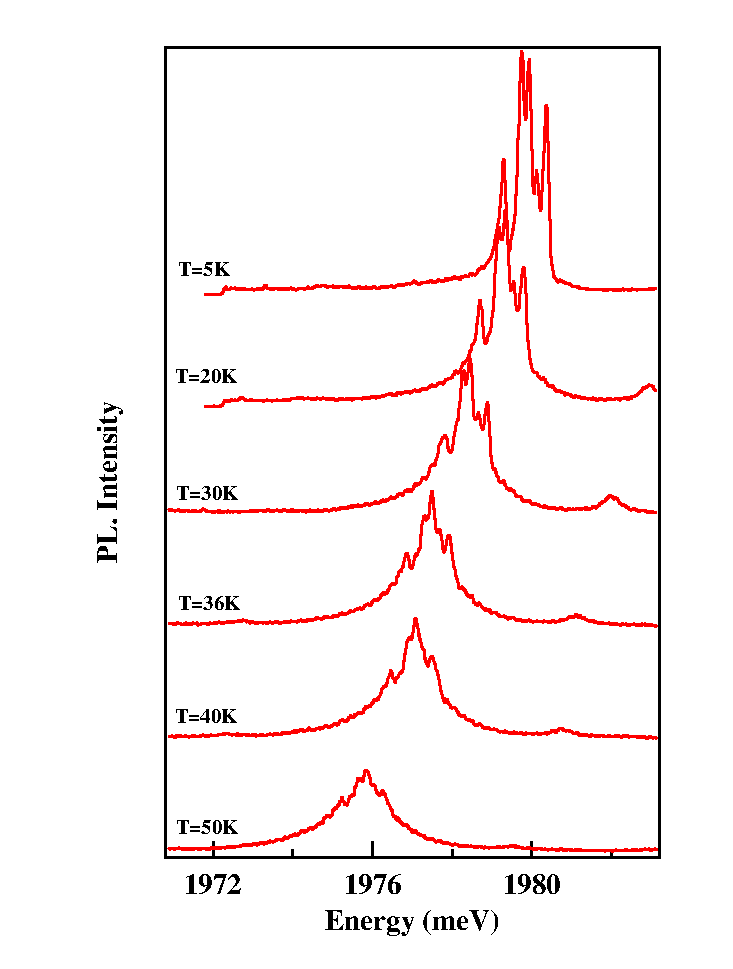
\includegraphics[width=2.75in]{FigS2.eps}
      \caption{Temperature dependence of the photoluminescence of X-Cr in a Cr-doped QD (QD4 in the main text).}
      \label{FigS2}}
   \end{minipage} \hfill
   \begin{minipage}[c]{.48\linewidth}
      \centering{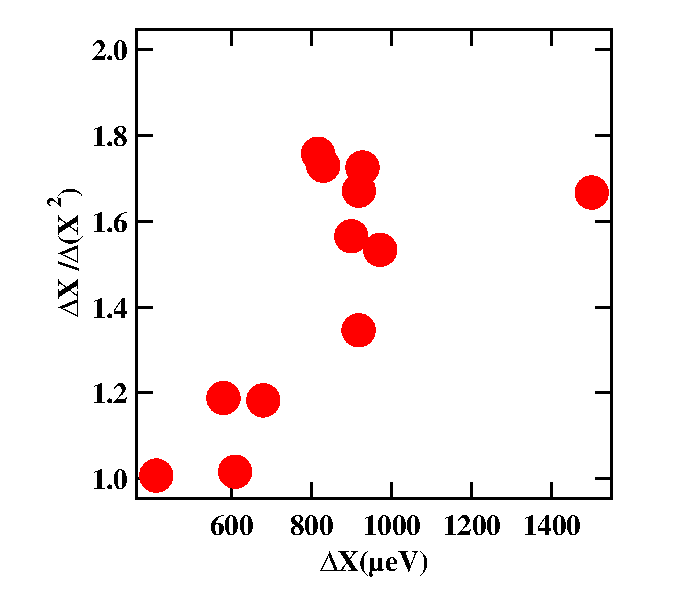
\includegraphics[width=2.5in]{FigS3.eps}
      \caption{Ratio of the overall splitting (i.e energy difference between the two extreme bright exciton lines) of X$^2$-Cr and X-Cr as a function of the splitting of X-Cr for 12 different Cr-doped QDs.}
      \label{FigS3}}
   \end{minipage}
\end{figure}

Figure \ref{FigS3} presents some statistics on the values of the overall energy splitting of X-Cr ($\Delta X$) and X$^2$-Cr ($\Delta X^2$) obtain on 12 Cr-doped quantum dots. For most of the investigated dots, $\Delta X$ remains below 1 meV and $\Delta X^2$ is also smaller than $\Delta X$ suggesting an interaction between the Cr spin and the biexciton.

\begin{thebibliography}{}

\bibitem{Vallin1974} J.T. Vallin and G.D. Watkins, Phys. Rev. B {\bf 9}, 2051 (1974).
\bibitem{Brousseau1988} M. Brousseau, Les defauts ponctuels dans les semiconducteurs, Les Editions de Physiques (1988).
\bibitem{Greenough1973} R.D. Greenough, S.B. Palmer, J. Phys. D {\bf 6}, 586 (1973).
\bibitem{Ovar2014} P. Ovartchaiyapong, K. W. Lee, B. A. Myers, A. C. Bleszynski Jayich, Nature Communication {\bf 5}, 4429 (2014).
\bibitem{Zielinski2015} M. Zielinski, Y. Don and D. Gershoni, Phys. Rev. B {\bf 91}, 085403 (2015).
\bibitem{Bayer2002} M. Bayer, G. Ortner, O. Stern, A. Kuther, A.A. Gorbunov, A. Forchel, P. Hawrylak, S. Fafard, K. Hinzer, T.L. Reinecke, S.N. Walck, J.P. Reithmaier, F. Klopf, F. Schafer, Phys. Rev. B {\bf 65}, 195315 (2002).
\bibitem{Leger2007} Y. Leger, L. Besombes, L. Maingault, H. Mariette, Phys. Rev. B {\bf 76}, 045331 (2007).
\bibitem{Besombes2014} B. Varghese, H. Boukari, L. Besombes, Phys. Rev. B {\bf 90}, 115307 (2014).
\bibitem{Besombes2005} L. Besombes, Y. Leger, L. Maingault, D. Ferrand, H. Mariette, J. Cibert, Phys. Rev. B {\bf 71}, 161307(R) (2005).
\bibitem{Trojnar2013} A. H. Trojnar, M. Korkusinski, U. C. Mendes, M. Goryca, M. Koperski, T. Smolenski, P. Kossacki, P. Wojnar, P. Hawrylak, Phys. Rev. B {\bf 87}, 205311 (2013).

\end{thebibliography}

\end{document}
